%!TEX program = lualatex

\documentclass[]{beamer} % notes, notes=only

\usetheme{EastLansing}
\usecolortheme{seagull}
\useinnertheme{rectangles}
\usefonttheme{professionalfonts}

\usepackage[utf8]{inputenc}
\usepackage[T1]{fontenc}

\usepackage{libertine}

\setmainfont[Ligatures=TeX]{Linux Biolinum O}


\AtBeginSection{\sectionpage}


\title[]{Working with Literature}
\author{https://github.com/aaaaalbert}
%\institute[]{}
\subtitle[]{--- DRAFT ---}
\date[]{2022-08-08\\\tiny CC BY-SA 4.0 (for non-draft versions)}


\usepackage[]{todonotes}
\newcommand{\topic}[1]{\todo[inline,color=blue!10]{Topic sentence: #1}}\newcommand{\albert}[1]{\todo[inline,color=red!10]{Albert: #1}}



\begin{document}


\frame{\titlepage}

%%%%%%%%%%%%%%%%%%%%%%%%%%%%%%%%%%%%%%%%%%%%%%%%%%%%%%%%%%%%%%%%%%%%%%%%
%
% \begin{frame}
% \frametitle{Outline}
% \framesubtitle{(optional)}
% 	\tableofcontents
% \begin{itemize}
%	\item ...
% \end{itemize}
% \end{frame}
% \note[itemize] {
% 	\item YOUR NOTE(S) HERE
% }
%%%%%%%%%%%%%%%%%%%%%%%%%%%%%%%%%%%%%%%%%%%%%%%%%%%%%%%%%%%%%%%%%%%%%%%%

%%%%%%%%%%%%%%%%%%%%%%%%%%%%%%%%%%%%%%%%%%%%%%%%%%%%%%%%%%%%%%%%%%%%%%%%
\begin{frame}
\frametitle{Motivation for this lecture}
\topic{Working with literature is an important fundamental skill in research}
\begin{itemize}
	\item You already know and do most of this anyway.
	\item We make stuff \alert{explicit} here so that we can reason about it.
\end{itemize}
\albert{Rework slide title. What do we actually want to say?}
\end{frame}
\note[itemize] {
	\item Probably no earth-shattering news here, because you are experienced to some degree:
	\item Bachelor's students → ``Vorwissenschaftliche Arbeit''
	\item Master's students → Bachelor's thesis
	\item PhD students → paper reading /reviews / writing
}
%%%%%%%%%%%%%%%%%%%%%%%%%%%%%%%%%%%%%%%%%%%%%%%%%%%%%%%%%%%%%%%%%%%%%%%%

%%%%%%%%%%%%%%%%%%%%%%%%%%%%%%%%%%%%%%%%%%%%%%%%%%%%%%%%%%%%%%%%%%%%%%%%
\begin{frame}
\frametitle{Student's natural motivation}
\framesubtitle{(Apologies for the hyperbole)}
I want to find (immediately, once and for all) literature that
\begin{itemize}
	\item proves my point
	\item suffices in extent, timeliness, recognition %in the field
	\item satisfies all formal requirements
	\item makes advisors and assessors happy
\end{itemize}
\end{frame}
\note[itemize] {
	\item I know because I have been there.
	\item (We all have.)
}
%%%%%%%%%%%%%%%%%%%%%%%%%%%%%%%%%%%%%%%%%%%%%%%%%%%%%%%%%%%%%%%%%%%%%%%%

%%%%%%%%%%%%%%%%%%%%%%%%%%%%%%%%%%%%%%%%%%%%%%%%%%%%%%%%%%%%%%%%%%%%%%%%
\begin{frame}
\frametitle{More likely outcome}
You \alert{will} find and \alert{traverse} networks of
\begin{itemize}
	\item authors, teams, institutions 
	\item workshops, conferences, journals
	\item topic areas and divisions
	\item papers and references
\end{itemize}
Also, be aware that working with literature is a \alert{continuous iterative process}.
\end{frame}
%%%%%%%%%%%%%%%%%%%%%%%%%%%%%%%%%%%%%%%%%%%%%%%%%%%%%%%%%%%%%%%%%%%%%%%%


%%%%%%%%%%%%%%%%%%%%%%%%%%%%%%%%%%%%%%%%%%%%%%%%%%%%%%%%%%%%%%%%%%%%%%%%
\begin{frame}
\frametitle{Fundamental motivation}
\begin{itemize}
%	\item Progress often is piecemeal
	\item Scientific processes demand \alert{transparency} and \alert{traceability} of origins of thoughts so that the community can assess them independently
	\item ``Nothing up my sleeves''
	\item Give credit where it is due
	\item Compare: open-source software
\end{itemize}
\end{frame}
%%%%%%%%%%%%%%%%%%%%%%%%%%%%%%%%%%%%%%%%%%%%%%%%%%%%%%%%%%%%%%%%%%%%%%%%

%%%%%%%%%%%%%%%%%%%%%%%%%%%%%%%%%%%%%%%%%%%%%%%%%%%%%%%%%%%%%%%%%%%%%%%%
\begin{frame}
\frametitle{Scientific literature as a communication device}
\begin{itemize}
	\item ``Stand on the shoulders of giants'': learn jargon, methods, evaluation approaches
	\item Get inspiration and new ideas
	\item Make yourself heard among the research community
	\item Document your actions so that others, too, can stand on \alert{your} shoulders
\end{itemize}
\end{frame}
%%%%%%%%%%%%%%%%%%%%%%%%%%%%%%%%%%%%%%%%%%%%%%%%%%%%%%%%%%%%%%%%%%%%%%%%

%%%%%%%%%%%%%%%%%%%%%%%%%%%%%%%%%%%%%%%%%%%%%%%%%%%%%%%%%%%%%%%%%%%%%%%%
\begin{frame}
\frametitle{Qualities of sources}
\small
Sources generally may include newspapers, TV shows, Web etc. \cite{sacred-heart}. Sources for scientific use should provide:

\begin{itemize}
	\item Named authors
	\item Reliable ``track records'': Renowned publication medium and authors, proper application of scientific processes (including citations)
	\item Peer reviewed, Open Source, Open Data
	\item Stable content and identifiers; versioning
\end{itemize}
(Note different emphases in different fields, e.g. mathematics, biology, physics)
\end{frame}
\albert{Maybe rephrase title to segue better from earlier ``sci.lit.''}
\note[itemize] {
	\item ``Track record'' equals cold-start problem for newcomers
	\item Ergo, newcomers should ensure they absolutely follow best practices in their field
	\item Learn by reading a lot!
	\item Wikipedia is usually NOT considered a proper source for scientific use -- see ``authors'' part above. (This does not mean it is no useful resource, nor is plagiarism allowed because of that.)
	\item Not all published papers are good resources either. Check for errata, retractions, contradictions in other papers; also check ``surroundings'' of suspicious papers: venue, authors, teams, institutions...
}
%%%%%%%%%%%%%%%%%%%%%%%%%%%%%%%%%%%%%%%%%%%%%%%%%%%%%%%%%%%%%%%%%%%%%%%%

%%%%%%%%%%%%%%%%%%%%%%%%%%%%%%%%%%%%%%%%%%%%%%%%%%%%%%%%%%%%%%%%%%%%%%%%
\begin{frame}
\frametitle{Literature discovery cycle}
Schematic process for obtaining sources:
\begin{figure}
	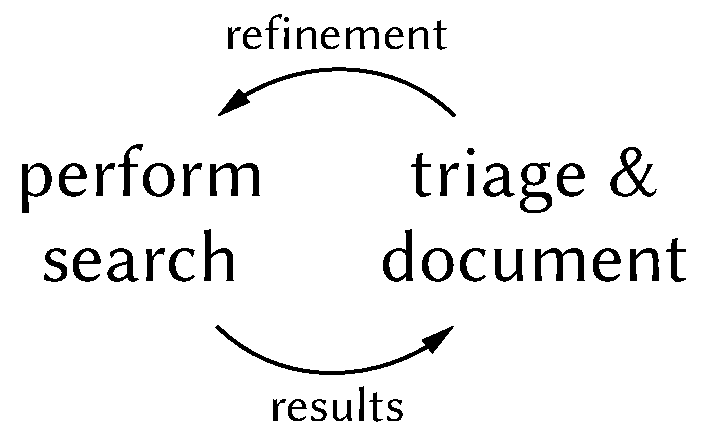
\includegraphics[width=0.4\textwidth]{fig/cycle.pdf}
	\label{fig:cycle}
\end{figure}
\begin{itemize}
	\item Perform a \alert{search} for the (approximate, assumed) topic
	\item \alert{Triage} the results: Keep good ones, discard others
	\item \alert{Document} what you found and why you kept or discarded it
	\item Perform another search with \alert{refined} parameters
	\item Repeat
\end{itemize}
\end{frame}
%%%%%%%%%%%%%%%%%%%%%%%%%%%%%%%%%%%%%%%%%%%%%%%%%%%%%%%%%%%%%%%%%%%%%%%%

%%%%%%%%%%%%%%%%%%%%%%%%%%%%%%%%%%%%%%%%%%%%%%%%%%%%%%%%%%%%%%%%%%%%%%%%
\begin{frame}
\frametitle{Efficient triage}
Problem: we cannot read every detail of every paper to determine relevance.

Solution: \alert{stepwise triage}. Perform simple checks on every search result, discard outliers at the earliest possible stage.
\begin{itemize}
	\item Title
	\item Abstract
	\item Publication format (poster, extended abstract, paper, article, book)
	\item Number and quality of references
	\item Conference or workshop venue, journal
	\item Authors, institutions, year of publication, citation count
\end{itemize}
→ A paper that we kept this far may be considered in depth.
\end{frame}
%%%%%%%%%%%%%%%%%%%%%%%%%%%%%%%%%%%%%%%%%%%%%%%%%%%%%%%%%%%%%%%%%%%%%%%%

%%%%%%%%%%%%%%%%%%%%%%%%%%%%%%%%%%%%%%%%%%%%%%%%%%%%%%%%%%%%%%%%%%%%%%%%
\begin{frame}
\frametitle{Refinement approaches}
Problem: Naïve search may yield too few / many results

Solutions to try out:
\begin{itemize}
	\item Choose (combination of) search terms, use proper terminology
	\item Sort and filter results
	\item ``Advanced'' search for specific properties
	\item Traverse author/institution/conference relationships: metadata is hyperlinked
\end{itemize}
Sometimes, grunt work is the way to go: skim / read a lot, throw away a lot
\end{frame}
\note[itemize] {
	\item A worked live example might be in order here.
	\item E.g. limit publication dates, search in title vs full text, traverse single conference's or author's history
	\item Don't run away yet, we need to talk about recording the results!
}
%%%%%%%%%%%%%%%%%%%%%%%%%%%%%%%%%%%%%%%%%%%%%%%%%%%%%%%%%%%%%%%%%%%%%%%%

%%%%%%%%%%%%%%%%%%%%%%%%%%%%%%%%%%%%%%%%%%%%%%%%%%%%%%%%%%%%%%%%%%%%%%%%
\begin{frame}
\frametitle{Search platforms}
\small
\begin{itemize}
	\item Typical first try: Web search
	\item Problem: does not turn up many ``proper'' sources
	\item Recommendation: use publishers' databases
	\item E.g. \href{https://dl.acm.org/}{ACM Digital Library}, \href{https://ieeexplore.ieee.org/}{IEEE Xplore}, \href{https://link.springer.com/}{Springer Link} (institutional login required, e.g \href{https://uaccess.univie.ac.at/}{u:access})
\end{itemize}
\end{frame}
\note[itemize] {
 	\item Google Scholar does find proper sources, but often alternative / ``inofficially'' shared versions too
 	\item Workarounds exist for users with no institutional affiliation, e.g. public library computers
}
%%%%%%%%%%%%%%%%%%%%%%%%%%%%%%%%%%%%%%%%%%%%%%%%%%%%%%%%%%%%%%%%%%%%%%%%

%%%%%%%%%%%%%%%%%%%%%%%%%%%%%%%%%%%%%%%%%%%%%%%%%%%%%%%%%%%%%%%%%%%%%%%%
\begin{frame}
\frametitle{Starting points for searching}
\begin{itemize}
	\item ``Cold start'': rough idea for search term
	\item Recommendations: personal, lectures and books, recognized conferences and journals
	\item ``Snowballing'': methodically traverse bibliographies of papers \cite{snowballing}
	\item Chance encounters
	\item \alert{All of the above}
\end{itemize}
\end{frame}
%%%%%%%%%%%%%%%%%%%%%%%%%%%%%%%%%%%%%%%%%%%%%%%%%%%%%%%%%%%%%%%%%%%%%%%%


%%%%%%%%%%%%%%%%%%%%%%%%%%%%%%%%%%%%%%%%%%%%%%%%%%%%%%%%%%%%%%%%%%%%%%%%
\begin{frame}
\frametitle{Practical considerations}
Usually, we perform multiple literature discovery cycles in parallel (no clear breadth/depth-first search):
\begin{itemize}
	\item Each result is a potential point for branching off
	\item Switch between them as you like
	\item ``Zoom in'' (or out) on various parameters: follow (sub)topics, authors and teams, conferences, ...
	\item Parallel cycles yield further ideas for refinement
\end{itemize}
\end{frame}
%%%%%%%%%%%%%%%%%%%%%%%%%%%%%%%%%%%%%%%%%%%%%%%%%%%%%%%%%%%%%%%%%%%%%%%%


%%%%%%%%%%%%%%%%%%%%%%%%%%%%%%%%%%%%%%%%%%%%%%%%%%%%%%%%%%%%%%%%%%%%%%%%
\begin{frame}
\frametitle{Better searching ≈ finding}
\begin{itemize}
	\item Good news: ``network of papers'' is quite dense
	\item Ergo, starting point does not matter too much
	\item ...but use your time wisely!
	\item Proper terminology makes a difference
	\item You will pick it up as you go
\end{itemize}
\end{frame}
%%%%%%%%%%%%%%%%%%%%%%%%%%%%%%%%%%%%%%%%%%%%%%%%%%%%%%%%%%%%%%%%%%%%%%%%


%%%%%%%%%%%%%%%%%%%%%%%%%%%%%%%%%%%%%%%%%%%%%%%%%%%%%%%%%%%%%%%%%%%%%%%%
\begin{frame}
\frametitle{WIP --- Record your findings}
\framesubtitle{...the smart way, lol}
\topic{See example paper truss}
\topic{Use LaTeX / BibTeX to manage workable lists of references (custom sorting, print all of the abstracts, add notes, ...}
\topic{The literature search and selection process deserves documentation as well!}
\end{frame}
%%%%%%%%%%%%%%%%%%%%%%%%%%%%%%%%%%%%%%%%%%%%%%%%%%%%%%%%%%%%%%%%%%%%%%%%

%%%%%%%%%%%%%%%%%%%%%%%%%%%%%%%%%%%%%%%%%%%%%%%%%%%%%%%%%%%%%%%%%%%%%%%%
\begin{frame}
\frametitle{WIP --- References and Further Reading}
\albert{BibTeXify this!}
\begin{itemize}
	\item Sacred Heart University Library \cite{sacred-heart}
	\item Snowballing paper \cite{snowballing}
\end{itemize}
\end{frame}
%%%%%%%%%%%%%%%%%%%%%%%%%%%%%%%%%%%%%%%%%%%%%%%%%%%%%%%%%%%%%%%%%%%%%%%%

%%%%%%%%%%%%%%%%%%%%%%%%%%%%%%%%%%%%%%%%%%%%%%%%%%%%%%%%%%%%%%%%%%%%%%%%
\end{document}

